\documentclass[12pt]{article}


\newcommand{\GroupId}{idk}
\newcommand{\assignment}{project-security}

\NeedsTeXFormat{LaTeX2e}
\usepackage[osf]{mathpazo}
\usepackage[svgnames]{xcolor}
\usepackage[T1]{fontenc}
\usepackage{amsmath,amsthm,amsfonts,amssymb,mathtools}
\usepackage{hyperref,url}
\usepackage[margin=2.7cm,a4paper]{geometry}
\usepackage{tasks}
\usepackage{xstring}
\usepackage[tikz]{mdframed}
\usepackage{environ}
\usepackage{etoolbox}
\usepackage{fourier-orns}
\usepackage{kvoptions}
\usepackage[]{units}
\usepackage{url}%
\usepackage[normal]{subfigure}

% math config

\DeclarePairedDelimiter\ceil{\lceil}{\rceil}
\DeclarePairedDelimiter\abs{\lvert}{\rvert}
\DeclarePairedDelimiter\set{\{}{\}}


% headers

\usepackage{fancyhdr}
\addtolength{\headheight}{2.5pt}
\pagestyle{fancy}
\fancyhead{} 
\fancyhead[L]{\sc info2222} % Replace with comp2123 or comp2823
\renewcommand{\headrulewidth}{0.75pt}

% update these headers
\fancyhead[C]{\sc Group Id: \GroupId}
\fancyhead[R]{Assignment \assignment}

\begin{document}

\section{Introduction}

This assignment is actually much better than Comp2017's o.O

\section{Approach explanation}
    \subsection*{Part: Basic Functionality Requirements:}
        \subsubsection*{1} Basically provided by template...

        \subsubsection*{2} King Zhou !!!

        \subsubsection*{3} King Zhou !!!

        \subsubsection*{5} 

        Users can click on a friend to open a chatroom. \textbf{King Zhou}\\

        \textbf{The process of ensuring secure communication between users:}
        \begin{enumerate}
            \item During the signup or login process, each user generates a pair of cryptographic keys: a public key and a private key. The public key is uploaded to the server and stored in a database called public\_keys, while the private key is retained in the user's local storage. These keys are generated based on the user's password, ensuring that they are consistently the same each time they are generated.
            \item For establishing a shared secret key, each party uses their own private key and the other party's public key to compute a value using elliptic curve cryptography (ECC). Despite the involvement of individual private keys and the corresponding public key, both parties arrive at the same shared secret key.
            \item This key is then used for symmetric encryption, enabling encrypted communication between the two. Symmetric encryption, which utilizes the same key for both encryption and decryption, is faster than asymmetric encryption and is well-suited for encrypting large volumes of data.
        \end{enumerate}



    \subsection*{Part: Additional Criteria:}

        \subsubsection*{1} When signing up, after checking if the user has already signed up, the server will generate a random salt and hash the password with this salt. Finally, it stores the username, salt, and hashed password in the database.

        \begin{figure}[h]
            \centering
            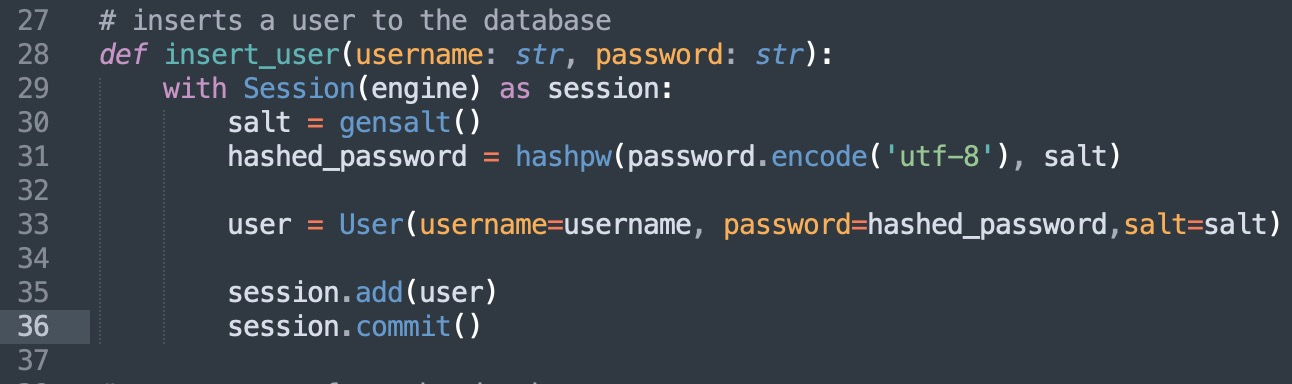
\includegraphics[width=0.8\textwidth]{graphs/insert_user.jpg}
            \caption{db.py insert\_user()}
        \end{figure}

        \begin{figure}[h]
            \centering
            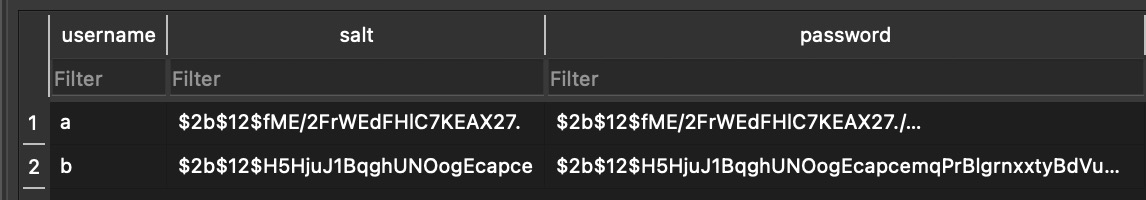
\includegraphics[width=0.8\textwidth]{graphs/hashed_passwd.jpg}
            \caption{main.db Table: user}
        \end{figure}



\section{Contribution}

        \begin{verbatim}
            #include <iostream>

            int main() {
                std::cout << "Hello, World!" << std::endl;
                return 0;
            }
        \end{verbatim}

\end{document}